% rep: representação
% reta: reta real
% A: intervalo aberto
% F: intervalo fechado
% Inf: infinito

\newcommand{\repretaAA}{
\vspace{0pt}
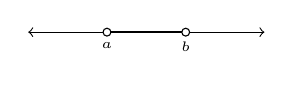
\begin{tikzpicture}[baseline]
    \draw[<->] (0, 0) -- (3, 0);
    \draw[thick] (1, 0) -- (2,0);

    \draw[fill=white] (1, 0) circle (0.05cm);
    \draw node[below=0.1pt, black] at (1, 0) {\tiny $a$};

    \draw[fill=white] (2, 0) circle (0.05cm);
    \draw node[below=0.1pt, black] at (2, 0) {\tiny $b$};
    
\end{tikzpicture}%
}

\newcommand{\repretaAF}{
\vspace{0pt}
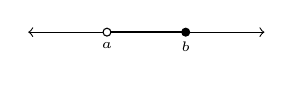
\begin{tikzpicture}[baseline]
    \draw[<->] (0, 0) -- (3, 0);
    \draw[thick] (1, 0) -- (2,0);

    \draw[fill=white] (1, 0) circle (0.05cm);
    \draw node[below=0.1pt, black] at (1, 0) {\tiny $a$};

    \draw[fill=black] (2, 0) circle (0.05cm);
    \draw node[below=0.1pt, black] at (2, 0) {\tiny $b$};
    
\end{tikzpicture}%
}

\newcommand{\repretaFA}{
\vspace{0pt}
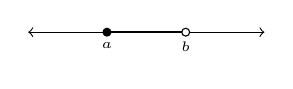
\begin{tikzpicture}[baseline]
    \draw[<->] (0, 0) -- (3, 0);
    \draw[thick] (1, 0) -- (2,0);

    \draw[fill=black] (1, 0) circle (0.05cm);
    \draw node[below=0.1pt, black] at (1, 0) {\tiny $a$};

    \draw[fill=white] (2, 0) circle (0.05cm);
    \draw node[below=0.1pt, black] at (2, 0) {\tiny $b$};
    
\end{tikzpicture}%
}

\newcommand{\repretaFF}{
\vspace{0pt}
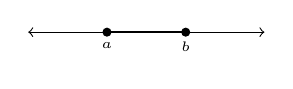
\begin{tikzpicture}[baseline]
    \draw[<->] (0, 0) -- (3, 0);
    \draw[thick] (1, 0) -- (2,0);

    \draw[fill=black] (1, 0) circle (0.05cm);
    \draw node[below=0.1pt, black] at (1, 0) {\tiny $a$};

    \draw[fill=black] (2, 0) circle (0.05cm);
    \draw node[below=0.1pt, black] at (2, 0) {\tiny $b$};
    
\end{tikzpicture}%
}

\newcommand{\repretaAInf}{
\vspace{0pt}
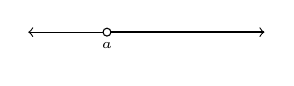
\begin{tikzpicture}[baseline]
    \draw[<->] (0, 0) -- (3, 0);
    \draw[thick] (1, 0) -- (3,0);

    \draw[fill=white] (1, 0) circle (0.05cm);
    \draw node[below=0.1pt, black] at (1, 0) {\tiny $a$};
\end{tikzpicture}%
}

\newcommand{\repretaFInf}{
\vspace{0pt}
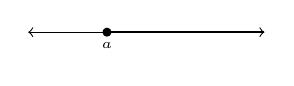
\begin{tikzpicture}[baseline]
    \draw[<->] (0, 0) -- (3, 0);
    \draw[thick] (1, 0) -- (3,0);

    \draw[fill=black] (1, 0) circle (0.05cm);
    \draw node[below=0.1pt, black] at (1, 0) {\tiny $a$};
\end{tikzpicture}%
}

\newcommand{\repretaInfA}{
\vspace{0pt}
\begin{tikzpicture}[baseline]
    \draw[<->] (0, 0) -- (3, 0);
    \draw[thick] (0, 0) -- (1,0);

    \draw[fill=white] (1, 0) circle (0.05cm);
    \draw node[below=0.1pt, black] at (1, 0) {\tiny $a$};
\end{tikzpicture}%
}

\newcommand{\repretaInfF}{
\vspace{0pt}
\begin{tikzpicture}[baseline]
    \draw[<->] (0, 0) -- (3, 0);
    \draw[thick] (0, 0) -- (1,0);

    \draw[fill=black] (1, 0) circle (0.05cm);
    \draw node[below=0.1pt, black] at (1, 0) {\tiny $a$};
\end{tikzpicture}%
}
